\documentclass{article}
\usepackage[margin=1.5cm,bottom=2cm]{geometry}
\usepackage{fancyhdr}
\usepackage{graphicx}
\usepackage[section]{placeins}
\pagestyle{fancy}
\usepackage{hyperref}
\usepackage[export]{adjustbox}
\pagestyle{fancy}
\usepackage{amsmath}
\usepackage{xcolor}
\hypersetup{colorlinks=true,urlcolor=blue,urlbordercolor=blue}
\begin{document}
\fancyhead[L]{ 
\includegraphics[width=2cm]{au_logo.png} }
\fancyhead[R]{ENGR 2310: Computational Problem Solving}
\fancyfoot[C]{\thepage}
\vspace*{0cm}
\begin{center}
	{\LARGE \textbf{Project 1}}\\
	\vspace{.25cm}
	{\Large Estimating the value of Pi using Monte Carlo Integration}
	%\vspace{0.25cm}
	%{\Large Due: Friday, September 4}
\end{center}

In belated honor of $\pi$ day, this project will introduce you to a novel way to write a computer program to estimate the value of $\pi$. We will do this using little more than a random number generator.

\section*{Methodology}
\subsection*{Monte Carlo Integration}
Consider the two rectangles in Figure \ref{rect}. I want to randomly select a point $<x,y>$ from anywhere within the outer rectangle (including the inside of the inner rectangle), so that every point is equally likely to be selected. What is the probability that this point will \textit{also} lie within the inner rectangle? It turns out that it depends on the ratio of the area of the two rectangles:
\begin{equation*}
P(<x,y> \mathrm{inside\ inner\ rectangle})=\frac{\mathrm{area\ of\ inner}}{\mathrm{area\ of\ outer}}
\end{equation*}
Our intuition supports this. If the inner rectangle is very small compared to the outer one, then it is highly unlikely that the randomly selected point will also appear within the inner rectangle. Conversely, if the inner rectangle is nearly the same size as the outer one, it is very likely.

This logic is also useful the other way around. Suppose I know the area of the outer rectangle but not the area of the rectangle within. If I randomly select a point from anywhere within the outer rectangle, the probability that the point is also drawn from the inner rectangle is $P=A_\mathrm{inner}/A_\mathrm{outer}$. Even without knowing $A_\mathrm{inner}$, I can estimate $P$ by selecting not one but many points. Suppose I generate 100 different random $<x,y>$ points, and 75 of them originate from the inner rectangle. This tells me that $P(<x,y> \mathrm{inside\ inner\ rectangle})=75/100=0.75$. Since $P=A_\mathrm{inner}/A_\mathrm{outer}$, I can therefore say that the area of the inner rectangle is 0.75 times the area of the outer one, which I know. I have used a random number generator to find the area of the shape. This is an example of a computational technique known as Monte Carlo integration (in reference to the Monte Carlo casino in Monaco).

This example is rather trivial, since it is not hard to just calculate the area of the inner rectangle. The beauty of this technique is that it works for \textit{any} shape. Give me some weird unknown shape, and I can place it within a rectangle and use random numbers to estimate its area (Figure \ref{rect2}).

An obvious limitation of this method is that we can only ever \textit{estimate} $P=A_\mathrm{inner}/A_\mathrm{outer}$; we cannot use random numbers to calculate it exactly. Therefore, the value we find for $A_\mathrm{inner}$ is not exact. If you generate $N$ many points, then the estimate of $A_\mathrm{inner}$ is likely to be within $\frac{A_\mathrm{outer}}{\sqrt{N}}$ of the true value.
\begin{figure}[ht!]
	\centering
	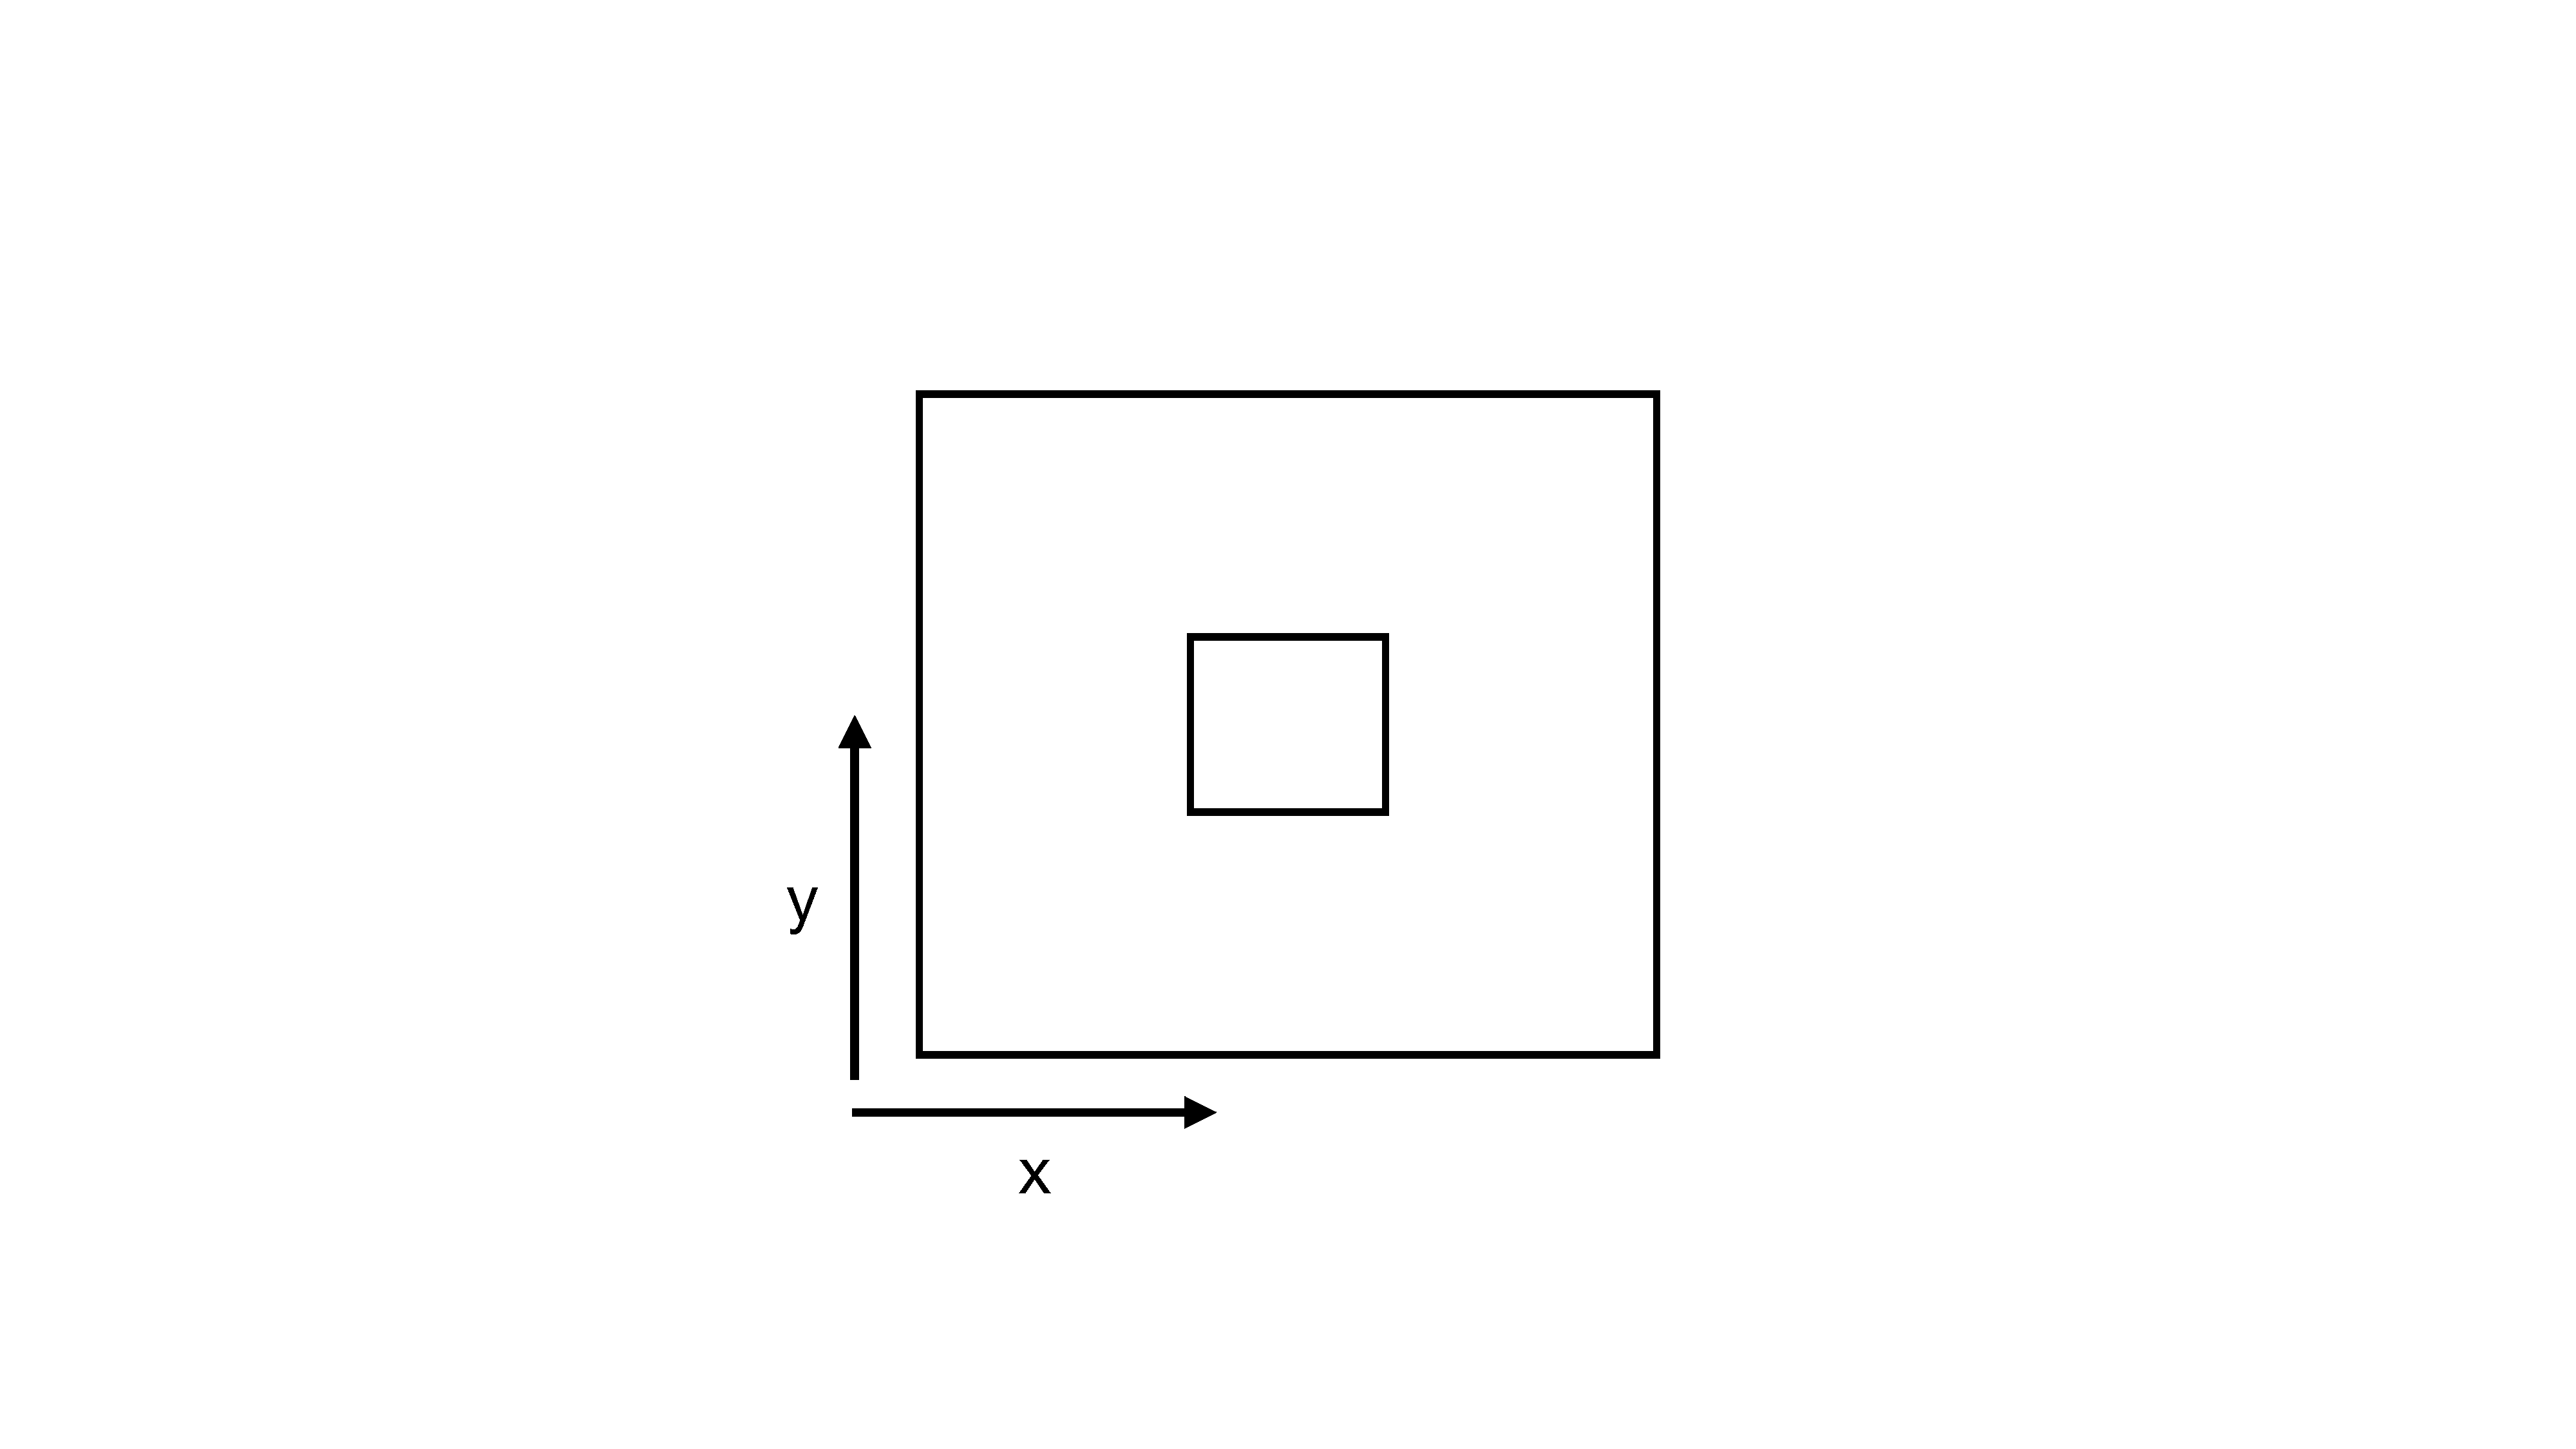
\includegraphics[width=0.5\textwidth]{mc_integral_fig}
	\caption{}
	\label{rect}
\end{figure}

\begin{figure}[ht!]
	\centering
	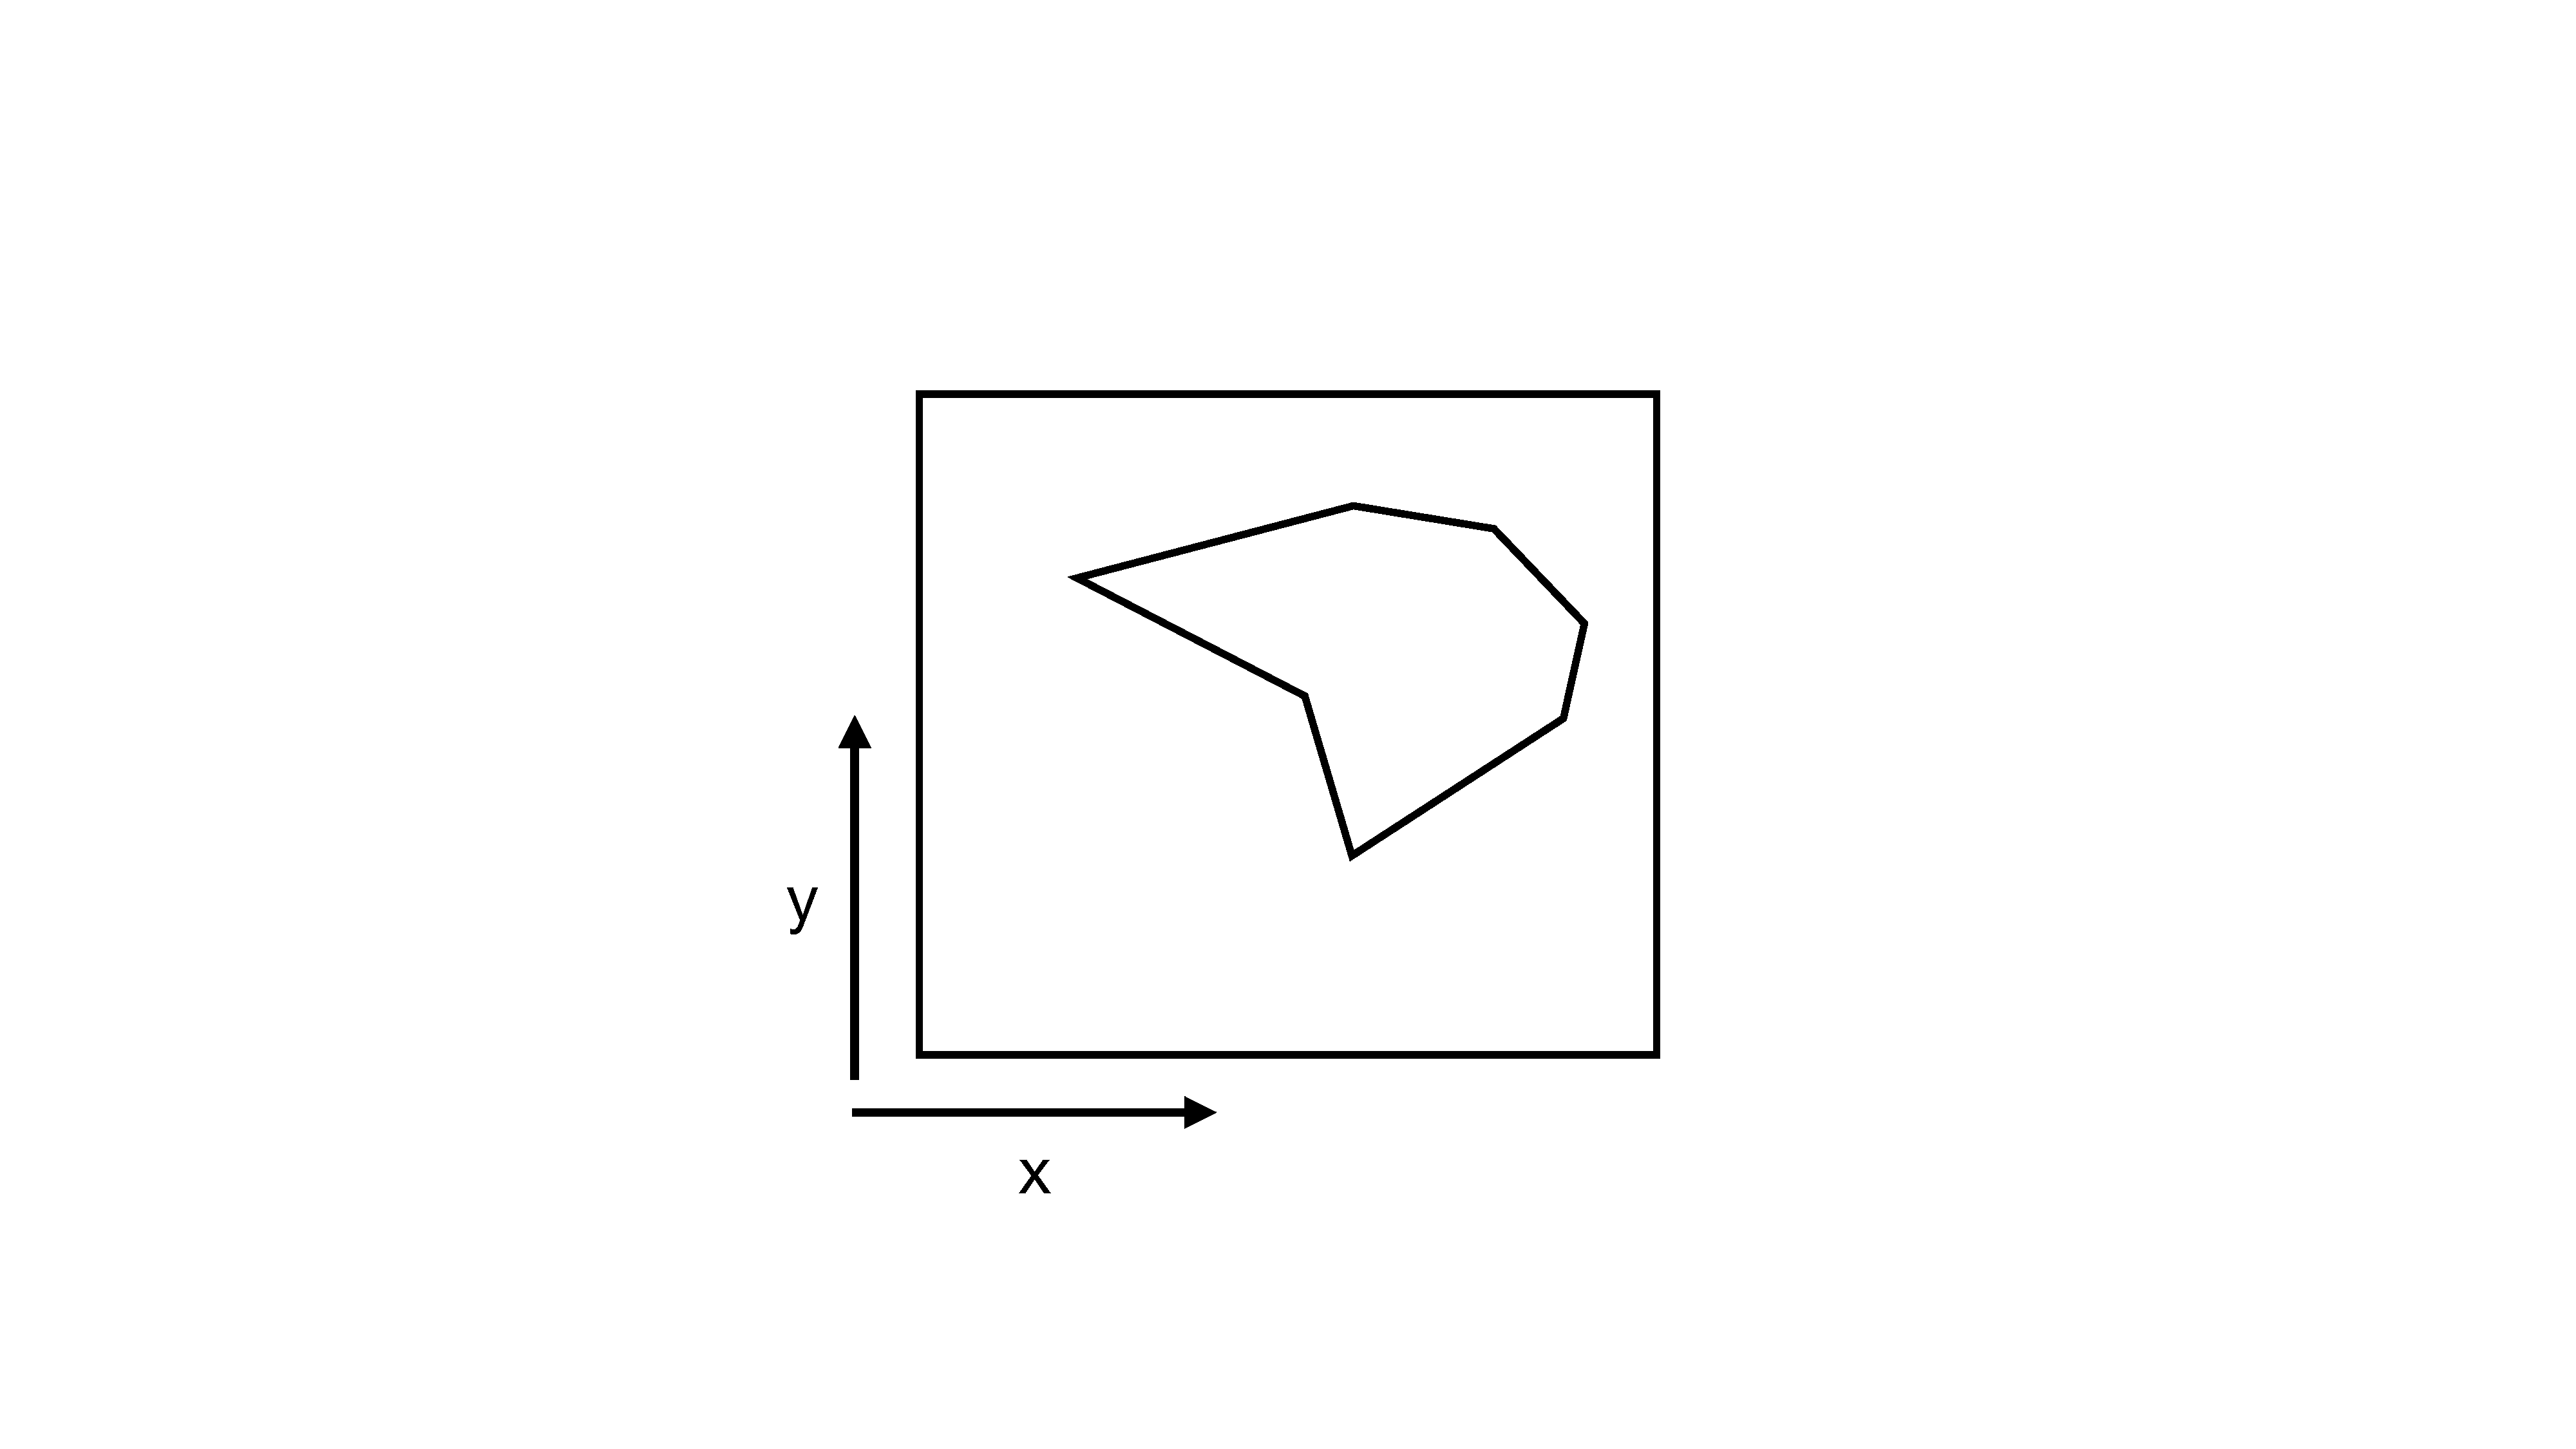
\includegraphics[width=0.5\textwidth]{mc_integral_fig_2}
	\caption{}
	\label{rect2}
\end{figure}

\section*{Project Description}
The goal of this project is use the Monte Carlo integration technique discussed in the previous section to estimate the area of a circle. If you then divide this area by the square of the radius of the circle, you will have an estimate of $\pi$. You will write code to do this several repeatedly while increasing the number of random points to explore how your estimate gets better with more random points.

To estimate the area, use the \texttt{random.uniform} function to generate a number of $<x,y>$ points drawn from a rectangle (or square). Then write code to determine what fraction of those points lie within the circle of radius $r$. Multiply this fraction by the area of the encompassing rectangle to estimate the area of the circle.
\subsection*{Details}
Your program should do the following:
\begin{itemize}
	\item Write a function called \texttt{inside\_circle(x,y,radius)} which returns \texttt{True} if the point \texttt{x,y} is located within the circle of radius \texttt{radius} (centered at the origin), and \texttt{False} otherwise
	\item Write a function called \texttt{estimate\_area(radius,N,l,w)} which generates $N$-many random points, drawn from a rectangle with width \texttt{l} and width \texttt{w}. The function should call \texttt{inside\_circle(x,y,radius)} on each point to determine if it is within the circle, and then estimate the area as discussed in the previous section. The function should return both the area and the quantity $\Delta A=\frac{lw}{\sqrt{N}}$, which is the uncertainty of your area estimate
	\item Finally, write the function \texttt{estimate\_pi(N,radius,l,w)} which calls \texttt{estimate\_area(radius,N,l,w)} and returns two things: a) the area divided by radius squared, and b) $\Delta A / r^2$, the approximate uncertainty on your estimate of $\pi$.
	\item In \texttt{main()}, ask the user which mode they want the program to run
	\begin{itemize}
		\item If the first mode is chosen, the program will then ask the user how many points to use for the estimation, and then use this value for $N$ to estimate pi and print the result and uncertainty. Note that the precision of your answer is limited to $1/N$; that is: the number of digits in your answer should equal the number of digits in $N$. Python's built in \texttt{round} function can help you with this.
		\item If the second mode is chosen, the program will estimate $\pi$ for several different values of $N$ and then plot $\pi$ vs $N$. The user will provide three numbers: $N_{min}$, $N_{max}$, and $n$, the number of points to include on the plot. Your program will estimate $\pi$ at $N_{min}$ and $N_{max}$, and $n-2$ many points in between, so that the number of points on the graph is $n$.
	\end{itemize}
\end{itemize}

\end{document}